\section{Hardware Testing}
The hardware is being tested on using the Diligent's Zybo board wic has
the Zynq 7010 SoC. This is a fairly small FPGA, hence the synthesized hardware 
can not be too large. The hardware being tested has the configuration as mentioned in the table 
\ref{tab:res:hwTesting:hwConfig}. 

\begin{figure}[H]
    \centering
    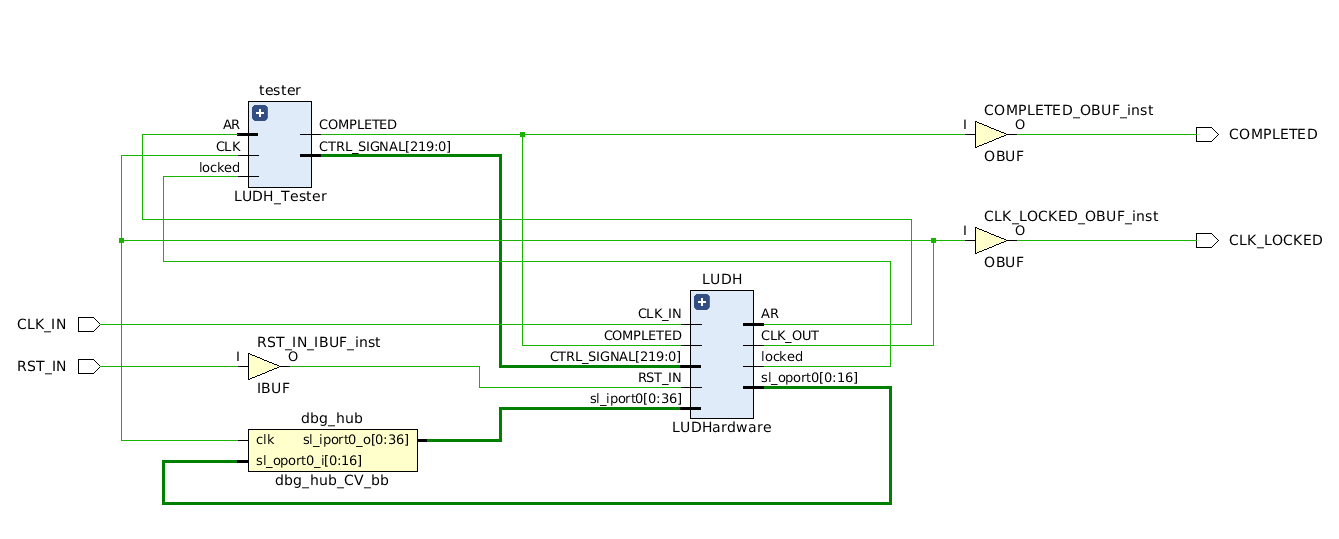
\includegraphics[width = 0.9\linewidth]{./Results/synHardware.png}
    \caption{Schematic of the synthesized hardware}
    \label{fig:res:synHwdd}
\end{figure}

For testing purposes the hardware is wrapped inside a synthesizable test bench 
which includes instruction and input matrix storage. This testbench emulates 
the behavior of master and main memory. 

\begin{table}[H]
    \centering
    \caption{Hardware configuration testing on FPGA}
    \label{tab:res:hwTesting:hwConfig}
    \begin{tabular}{L{6cm} L{1.5cm}}
        \toprule
        Parameter & Value \\
        \midrule
        Number of PEs           & 4  \\
        Number of BRAMs         & 4         \\
        Number of Ports/ BRAM   & 4         \\
        Read Latency of BRAM    & 2          \\
        Latency of MAC Unit     & 20          \\
        Latency of Divider Unit & 31          \\
        \bottomrule
    \end{tabular}
\end{table}


The operating frequency of the system is 
set at 100 MHz and it is generated using the PLL as mentioned in the hardware section.
The hdl generation tool also generate additional board files to incorporate
Hardware Integrated Logic Analyzer to debug and capture the on-chip waveforms.

At this stage all the components of the hardware except Quad Port BRAMs are working 
properly. The figure \ref{fig:res:synHwdd} shows the schematic of synthesized hardware.


\begin{figure}
    \centering
    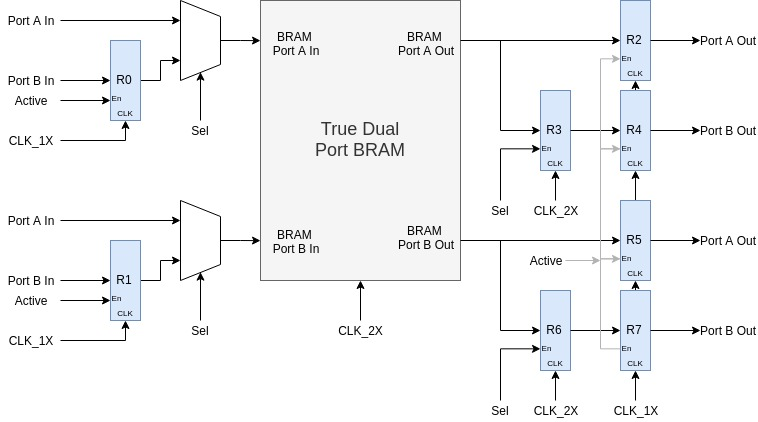
\includegraphics[width = 0.9\linewidth]{./Results/quadPortBRAM.jpg}
    \caption{BRAM unit with 4 time multiplexed ports}
    \label{fig:res:bram}
\end{figure}

\begin{figure}
    \centering
    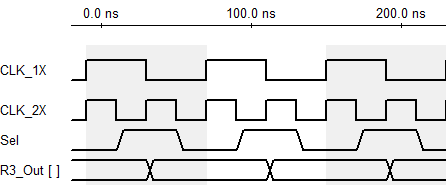
\includegraphics[width = 0.9\textwidth]{./Results/bramWaveProblem.png}
    \caption{Location of false hold violation}
    \label{fig:res:wave}
\end{figure}

\textbf{The Problem}\\
As we have discussed in the previous chapters the time multiplexed ports requires 
two separate clock sources with the ratio of operating frequencies 2:1. The figure 
\ref{fig:res:bram} shows the structure of the BRAM. If we look at the path between
registers $R3$ and $R4$, the path is sensitized by the faster clock and it 
acts as the input for the path in slower clock domain. As we have seen from the 
waveforms before, there is nothing wrong with this because the output of the 
register $R3$ is not going to change when $R4$ samples it because the $Sel$ signal
is low at the rising edge of the slower clock. But the timing analyzer flags it for the 
hold violation as it assumes that the output of $R3$ is going to change at every clock
cycle. 







\begin{figure}
    \centering
    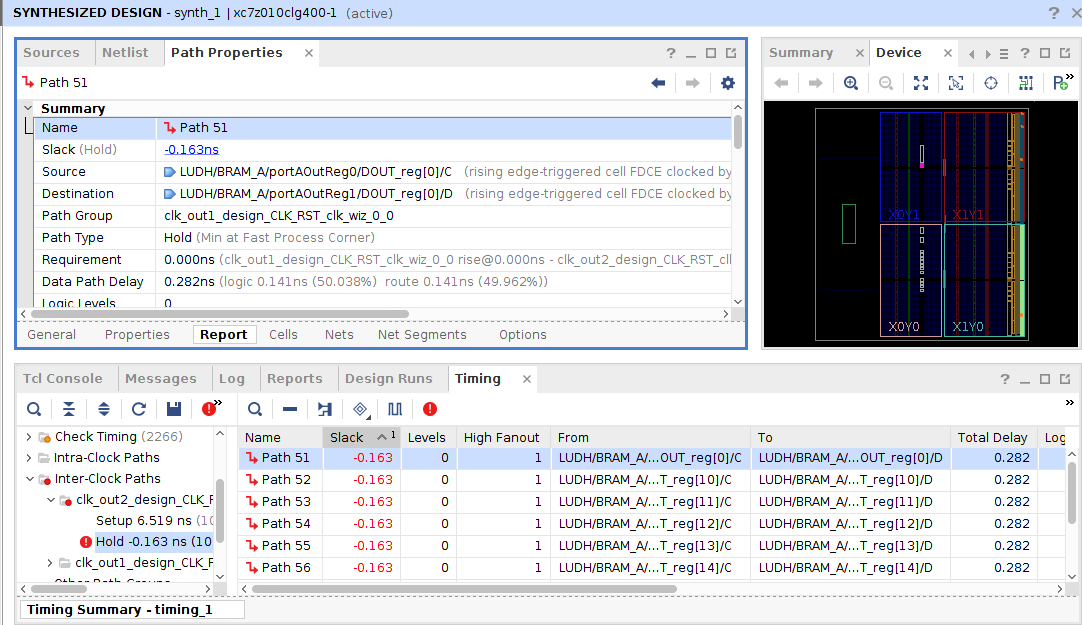
\includegraphics[width = \linewidth]{./Results/timingRepor.png}
    \caption{Hold violation reported by the synthesis tool}
    \label{fig:res:bram}
\end{figure}


